\documentclass{article}
\usepackage{tikz}
	\usetikzlibrary{shapes,arrows,shadows}
	\usetikzlibrary{decorations.pathmorphing}
	\usetikzlibrary{positioning}
	\usetikzlibrary{fit}
	\usetikzlibrary{trees} % for grow cyclic

\begin{document}
\setlength{\parindent}{0pt}
\setlength{\parskip}{1em}
\newcommand{\type}[1]{\mbox{\texttt{#1}}}
\newenvironment{maths}
{
    \vspace*{0.5em}
    \begin{tabular}{l}
}
{
    \end{tabular}
    \vspace*{1em}
}

\title{Use Cases to Predicates}
\author{Yegor Bugayenko\\\texttt{yegor@tpc2.com}}
\maketitle

\newpage
\section{Classes}

    Verbal form of a type/class (C++ as an example):

    \begin{verbatim}
User includes:
  email: "email address";
  photos: Photo-s "a collection of photos";
  manager: User "user's manager, if any";
  address includes: city, country, street.\end{verbatim}

    Formal ($\Pi_i$ is a set):
    
    \begin{maths}
    $\type{User}(x) :$ \\
    $\quad \exists \Pi_1 (|\Pi_1| = 1 \wedge$ \\
    $\quad\quad \forall p(p \in \Pi_1 \to $ \\
    $\quad\quad\quad \type{string}(p) \wedge$ \\
    $\quad\quad\quad \type{composition}(x, p) \wedge$ \\
    $\quad\quad\quad \type{info}(\mbox{``email address''})$ \\
    $\quad\quad ) $ \\
    $\quad ) \bigwedge $ \\
    $\quad \exists \Pi_2 (|\Pi_2| \geq 0 \wedge$ \\
    $\quad\quad \forall p(p \in \Pi_2 \to $ \\
    $\quad\quad\quad \type{Photo}(p) \wedge$ \\
    $\quad\quad\quad \type{composition}(x, p) \wedge$ \\
    $\quad\quad\quad \type{info}(\mbox{``a collection of photos''})$ \\
    $\quad\quad ) $ \\
    $\quad ) \bigwedge $ \\
    $\quad \exists \Pi_3 (|\Pi_4| < 2 \wedge $ \\
    $\quad\quad \forall p(p \in \Pi_4 \to $ \\
    $\quad\quad \type{User}(p) \wedge$ \\
    $\quad\quad \type{aggregation}(x, p) \wedge$ \\
    $\quad\quad \type{info}(\mbox{``user's manager, if any''})$ \\
    $\quad\quad ) $ \\
    $\quad ) \bigwedge $ \\
    $\quad \exists \Pi_4 (|\Pi_4| = 1 \wedge$ \\
    $\quad\quad \forall p(p \in \Pi_4 \to$ \\
    $\quad\quad\quad \exists \Psi_1(|\Psi_1|=1 \wedge \forall \psi(\psi \in \Psi_1 \to \type{string}(\psi) \wedge \type{composition}(p, \psi))) \wedge$ \\
    $\quad\quad\quad \exists \Psi_2(|\Psi_2|=1 \wedge \forall \psi(\psi \in \Psi_2 \to \type{string}(\psi) \wedge \type{composition}(p, \psi))) \wedge$ \\
    $\quad\quad\quad \exists \Psi_3(|\Psi_3|=1 \wedge \forall \psi(\psi \in \Psi_3 \to \type{string}(\psi) \wedge \type{composition}(p, \psi)))$ \\
    $\quad\quad ) $ \\
    $\quad )$ \\
    \end{maths}
    
    There are a number of sub-predicates:

    \begin{maths}
    $\type{User.email}(x, \Pi) = (|\Pi| = 1 \wedge \forall p(p \in \Pi \to \type{string}(p) \wedge \type{composition}(x, p))$ \\
    \end{maths}
    
\newpage
\section{Use Cases}

    Verbal form of a use case:
    
    \begin{verbatim}
    UC1: User (the user) extends photo album:
      1. The user creates photo of himself (the photo).
      2. We validate the photo "immediately".
      3. "We protocol the operation in backlog".
      4. The user reads the photo.
    UC1: 0a) If number of photos of the user is greater than 5:
      1. The user deletes photo of himself.
    UC1: 2a) If failed with "file format is not valid":
      1. We delete the photo.
      2. Fail with "only PNG images are accepted".\end{verbatim}

    Every use case is a predicate, $\type{UC}_1(x) = true$ means that the user
    successfully extended his photo album:
    
    \begin{maths}
    $\type{UC}_1(x) : $ \\
    $\quad \type{User}(x) \to$ \\
    $\quad \exists \Pi(\type{User.photos}(x, \Pi)) \to$ \\
    $\quad ($ \\
    $\quad\quad |\Pi| > 5 \wedge \type{info}(\mbox{``If number of photos of the user is greater than 5''})\to$ \\
    $\quad\quad \exists y(y \in \Pi) \to$ \\
    $\quad\quad \type{deleted}(y) \wedge \type{info}(\mbox{``The user deletes photo of himself''})$ \\
    $\quad ) \to$ \\
    $\quad \exists p(p \in \Pi) \to$ \\
    $\quad \type{created}(p, x) \wedge \type{info}(\mbox{``The user creates photo of himself (the photo)''})\to$ \\
    $\quad \type{UC}_2(p) \wedge \type{info}(\mbox{``We validate the photo immediately''}) \vee$ \\
    $\quad ($ \\
    $\quad\quad \type{exception}(\mbox{``file format is not valid''}) \to$ \\
    $\quad\quad \type{deleted}(p) \wedge \type{info}(\mbox{``We delete the photo''})\to$ \\
    $\quad\quad \type{throw}(\mbox{``only PNG images are accepted''})$ \\
    $\quad ) \to$ \\
    $\quad \type{silent}(\mbox{``We protocol the operation in backlog''})$ \\
    $\quad \type{read}(p, x)\wedge \type{info}(\mbox{``The user reads the photo''})$ \\
    \end{maths}
    
\newpage
\section{Basic Predicates}

    Basic fundamental predicates:

    \begin{maths}
    $\type{info}(x) = true$ \\
    $\type{composition}(x, y) = \dots$ \\
    $\type{aggregation}(x, y) = \dots$ \\
    $\type{created}(x) = \dots$ \\
    $\type{deleted}(x) = \dots$ \\
    $\type{read}(x) = \dots$ \\
    $\type{exception}(x) = \dots$ \\
    $\type{throw}(x) = \dots$ \\
    \end{maths}

    Primitive types:

    \begin{maths}
    $\type{integer}(x) = \dots$ \\
    $\type{string}(x) = \dots$ \\
    $\type{float}(x) = \dots$ \\
    $\type{boolean}(x) = \dots$ \\
    \end{maths}


\newpage
\section{Parser, Validator, Metric Collector, etc.}

    \begin{tikzpicture}
        [node distance=8em]
        \node [draw] (yacc) {YACC};
        \node [draw, right of=yacc] (brokers) {C++ brokers};
        \node [draw, right of=brokers] (proxy) {Proxy};
        \node [draw, right of=proxy] (solm) {SOLM};
        \node [above right of=solm] (uml) {UML};
        \node [right of=solm] (lisp) {Lisp};
        \node [below right of=solm] (metrics) {Metrics};
        
        \draw [thick, ->] (yacc) -- (brokers);
        \draw [thick, ->] (brokers) -- (proxy);
        \draw [thick, ->] (proxy) -- (solm);
        \draw [dashed, ->] (solm) -- (uml);
        \draw [dashed, ->] (solm) -- (lisp);
        \draw [dashed, ->] (solm) -- (metrics);
    \end{tikzpicture}
    

    SOLM is a collection of \emph{formulas}:

    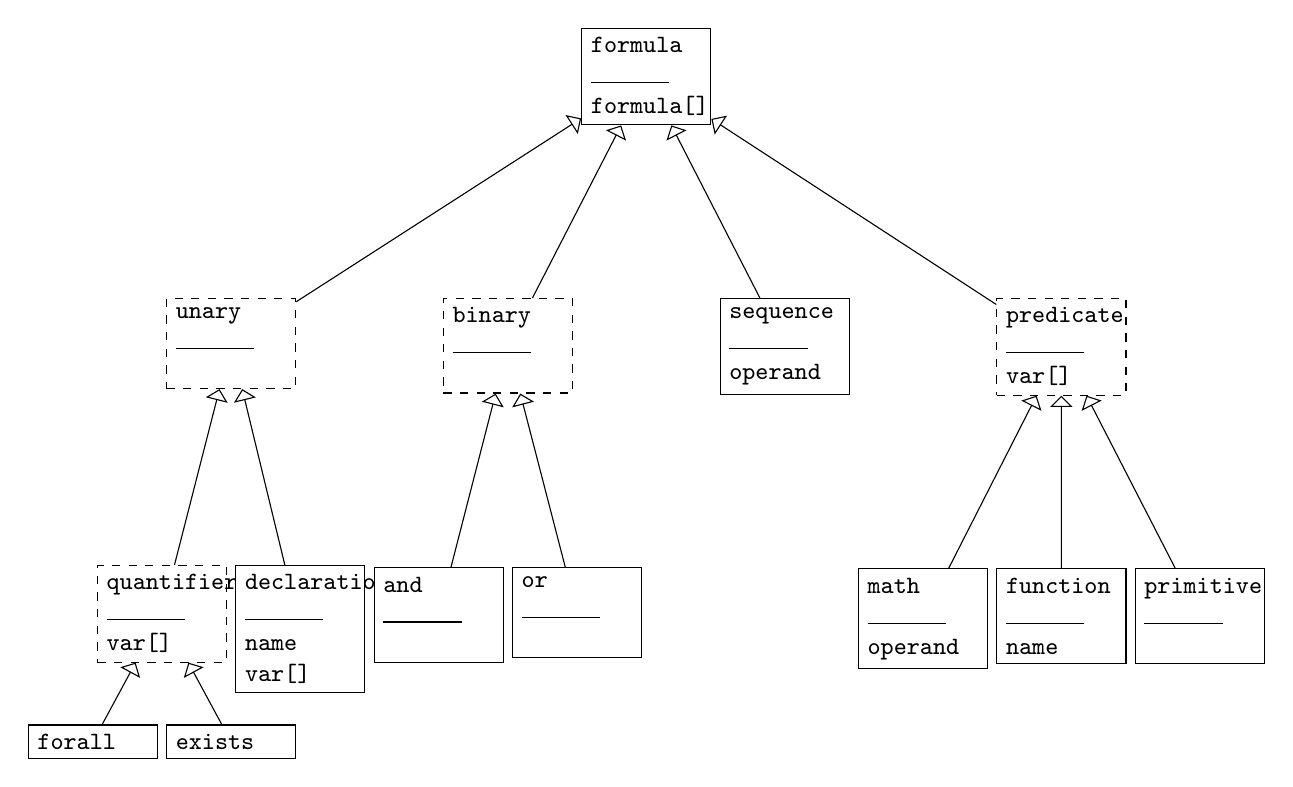
\begin{tikzpicture}[
        every node/.style={class},
        level 1/.style={level distance=8em, sibling distance=10em, open triangle 90-},
        level 2/.style={sibling distance=5em},
        ]
        \tikzstyle{class} = [draw, text width=4em, font={\small\ttfamily}, fill=white, anchor=north];
        \newcommand{\br}{\linebreak\rule{3em}{0.4pt}\linebreak}
        \node {formula\br formula[]}
            child {node [dashed] {unary\br}
                child {node [dashed] {quantifier\br var[]}
                    child [level distance=4em] {node {forall}}
                    child [level distance=4em] {node {exists}}
                }
                child {node {declaration\br name\linebreak var[]}} 
            }
            child {node [dashed] {binary\br}
                child {node {and\br}} 
                child {node {or\br}} 
            }
            child {node {sequence\br operand}} 
            child {node [dashed] {predicate\br var[]}
                child {node {math\br operand}}
                child {node {function\br name}}
                child {node {primitive\br}}
            }
        ;
    \end{tikzpicture}
    
    \clearpage
    Proxy is a collection of C++ classes:
    
    \begin{verbatim}
class Type {
  vector<solm::Formula*> predicates;
  vector<Slot> slots;
};
class Slot {
  string name;
  Cardinality cardinality;
  vector<solm::Formula*> predicates;
  Type* type;
};
map<string, Type> types; // all named types
class UseCase {
  class Signature {
    string format; // e.g. "${sud} validate ${photo}"
    map<string, Explanation> explanations; // e.g. <"photo", "User.photos">
  };
  Signature signature;
  typedef map<int, Flow> Flows;
  class Flow {
    string informal;
    Signature signature;
    map<solm::Formula*, Flows&> alternatives;
  };
};
\end{verbatim}

\end{document}
